\chapter{INTRODUCTION}
\vspace{5mm}
\section{Background and Motivation}
\noindent
Sustainable energy sources such as solar and wind power have become increasingly popular in the past decades \cite{Kiefer}. Combustion processes, however, are responsible for providing the majority of energy needs and remain vitally important in wide ranging applications such as electric generation, automotive power and spacecraft propulsion. Optimal utilization of limited fuel resources with reduced emissions requires a detailed understanding of combustion physics and chemistry, which is governed by complex and coupled multi-scale phenomenon including chemical kinetics, heat transfer and fluid dynamics. Non-invasive laser diagnostics play an important role in understanding combustion processes and thus reducing its impact on the environment \cite{Goldenstein2017, HANSON20111, Chang2018,  WOLFRUM19981,Allen1998, WERLE1998197, Lackner2007, Schulz2007, BOLSHOV201545, Eckbreth, Kohse, hanson2016spectroscopy}. 

Tunable diode-laser-absorption spectroscopy (TDLAS) sensors are one widely-used laser-diagnostic technique that offers great potential for non-intrusive, time-resolved and multi-parameter sensing in combustion systems \cite{Goldenstein2017}. These sensors have been used for performance testing, model validation and feedback control of combustors \cite{Goldenstein2017,Ma2013,Caswell2013,Stritzke2015,Witzel2013,Whitney2011,Makowiecki2017,Rieker2009b,Li2011}. During operation, laser light is transmitted through the test gas and collected on a photodetector. Gas conditions such as temperature and composition are then inferred by comparing the amount of light absorbed at specific wavelengths with that predicted by spectroscopic models. Direct absorption spectroscopy (DAS) and wavelength-modulation spectroscopy (WMS) are two of the most widely used and robust TDLAS techniques in both academic and industrial fields \cite{Lackner2007}.
 
Direct absorption is the simplest laser absorption spectroscopy technique. In DAS, laser light with given intensity and wavelength is directed through the test gas. A portion of the laser light can be absorbed by specific molecules if the photon energy is equal to the energy spacing between the molecule's internal quantized energy levels. In the infrared, absorption leads to molecules increasing from a lower rovibrational state (defined by a molecule existing in a specific rotational state and a specific vibrational state) to an upper rovibrational state. The amount of light transmitted through the gas is measured by photodetectors. The main drawback of DAS is that it is sensitive to non-absorbing transmission losses (e.g., from beamsteering, vibration, etc.). By contrast, wavelength-modulation spectroscopy (WMS) exhibits several noise-rejection benefits that can improve signal-to-noise (SNR) levels by a factor of 10-100 over DAS \cite{Rieker2009b}. Details of these two fundamental spectroscopy techniques are provided in the following chapters.

Historically, two main TDLAS sensor architectures have been used for gas-property measurements. The first type relies on optical access along a line-of-sight (LOS), where laser light is transmitted from one side and collected by a photodetector on the opposite side. The principle of this approach is simple, but not suitable in some practical environments with extremely limited optical access or in situations where stand-off detection is required. Recently, single-ended LAS (SE-LAS) sensors have been developed to address this problem and have emerged as a promising technology for characterizing combustion environments with limited optical access \cite{Goldenstein2017}. In this approach, laser light is backscattered off native surfaces \cite{Dubinsky1998, Wainner2002, Wang2015, Goldenstein:16, Peng:16, Peng2018} or mirrors inside optical probes \cite{RIEKER20073041, Rein:10, Chen2010, 0957-0233-25-11-115501, GIRARD2017158}. SE-LAS sensors have been used to make measurements of temperature in flames \cite{Goldenstein:16,Peng:16}, rotating-detonation engines \cite{Rein2017, Peng2018}, and internal combustion engines \cite{Melin2017}. The majority of this work has employed near-infrared wavelengths to interrogate the combination and overtone absorption bands of $H_2O$ using semiconductor lasers and telecommunication-grade fiber optics, however some work has been done using mid-infrared diode, interband-cascade and quantum-cascade lasers \cite{Peng2018, 0957-0233-25-11-115501, GIRARD2017158}. Most recently, Peng et al. \cite{Peng:16} developed a SE-LAS sensor operating in the mid-infrared to provide improved measurement sensitivity of $CO$, $CO_2$, and $H_2O$ via their stronger fundamental absorption bands. Peng et al. \cite{Peng2018} later used this sensor and WMS-$2f/1f$ to provide measurements of temperature and $H_2O$ at 20 $kHz$ in the annulus of a rotating-detonation engine.

SE-LAS sensors have been increasingly popular to characterize different combustion environments with limited optical access. However, all prior backscattering-based SE-LAS sensing in combustion environments relied on the uses of windows to isolate the sensor lens from high-temperature combustion gases. This increases sensor cost to some extent and can complicate sensor installation because care must be taken during alignment to avoid collecting strong reflections off the window surface which can significantly compromise the accuracy of single-ended LAS sensors. Similarly for SE-LAS sensors with protruding mirrors, heat transfer between gas and the probe body introduces significant temperature bias to the measurements \cite{Rein:10}. 

In this dissertation, the design of a compact SE-LAS sensor for measuring temperature and $H_2O$ concentration in high-temperature combustion environment is presented. This design builds on the fiber-coupled SE-LAS sensor developed previously by Goldenstein et al. \cite{Goldenstein:16} to provide several design improvements which increase the practicality and applicability of laser-absorption sensors without compromising measurement quality. The novelty of this sensor includes: (1) development of a windowless sensor architecture that can withstand direct exposure to high-temperature combustion gases for long durations (e.g., 30 min); (2) a compact \& rugged sensor housing that employs a single 6 mm diameter lens. The validation and application of this sensor is presented in temperature and $H_2O$ sensing in a propane-air burner (see Fig. 1.1).

\vspace{15mm}
\begin{figure}[ht]
    \centering
        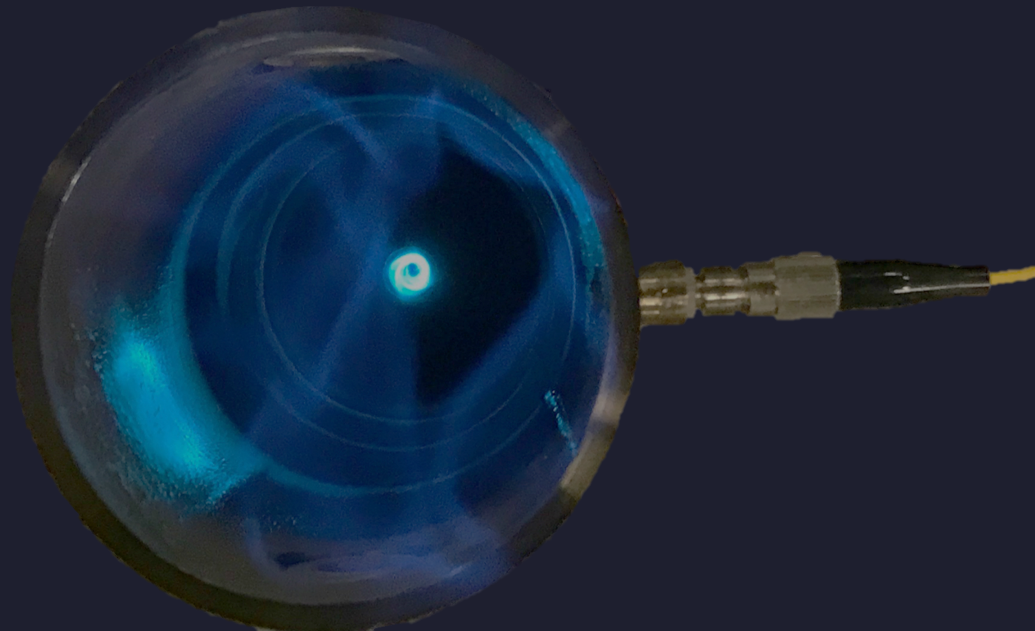
\includegraphics[width=0.55\textwidth]{fig/ch1_fig1.png}
        \caption{Single-ended LAS sensor for temperature and ${H_2}O$ measurements in a propane burner}
    \label{fig:ch1_1}
\end{figure}

\section{Review of the Literature}
\subsection{Traditional line-of-sight laser-absorption sensor}
The use of line-of-sight LAS in combustion is traced back to the late 1970s. In 1977, tunable diode lasers (TDLs) were applied to provide two-color thermometry in flame gases for the first time by Hanson \cite{Hanson19771479}. Since then, line-of-sight LAS sensors have been widely used to acquire path-averaged measurements of gas temperature, pressure, composition and velocity in countless combustion environments \cite{Goldenstein2017, HANSON20111, WOLFRUM19981,Allen1998, WERLE1998197, Lackner2007, Schulz2007, BOLSHOV201545, Eckbreth, Kohse, hanson2016spectroscopy}. 

To mention a few examples, Jatana et al. \cite{Jatana:15, Jatana2} made use of TDLs to achieve line-of-sight measurements of temperature, pressure and water concentration in the intake manifold and exhaust of a diesel engine. Mattison et al. \cite{Mattison2007} developed a wavelength-multiplexed line-of-sight LAS sensor to make crank-angle-resolved measurements of temperature and water concentration in a homogeneous-charge-compression-ignition (HCCI) engine (see Fig. 1.2). Fused-silica rings and windows were utilized in the top of the cylinder liner to provide a line-of-sight optical access in cylinder. In high-speed combustion flows, Goldenstein et al. \cite{goldenstein2014wavelength,goldenstein2014wavelength2} and Spearrin et al. \cite{spearrin1,spearrin2014quantum} employed mid-infrared LAS sensing of temperature, $H_2O$, $CO_2$ and $CO$ in scramjets and detonation engines \cite{goldenstein2015infrared}. Jackson et al. \cite{Jackson2015} presented a in-flight water-based measurements at the exit of the HIFiRE 2 scramjet combustor (see Fig. 1.3). Eight near-infrared (NIR) sensors were used to provide measurements across 5 vertical and 3 horizontal lines of sight. While very useful, these sensors are limited to applications that can provide line-of-sight optical access.

\begin{figure}[ht]
    \centering
        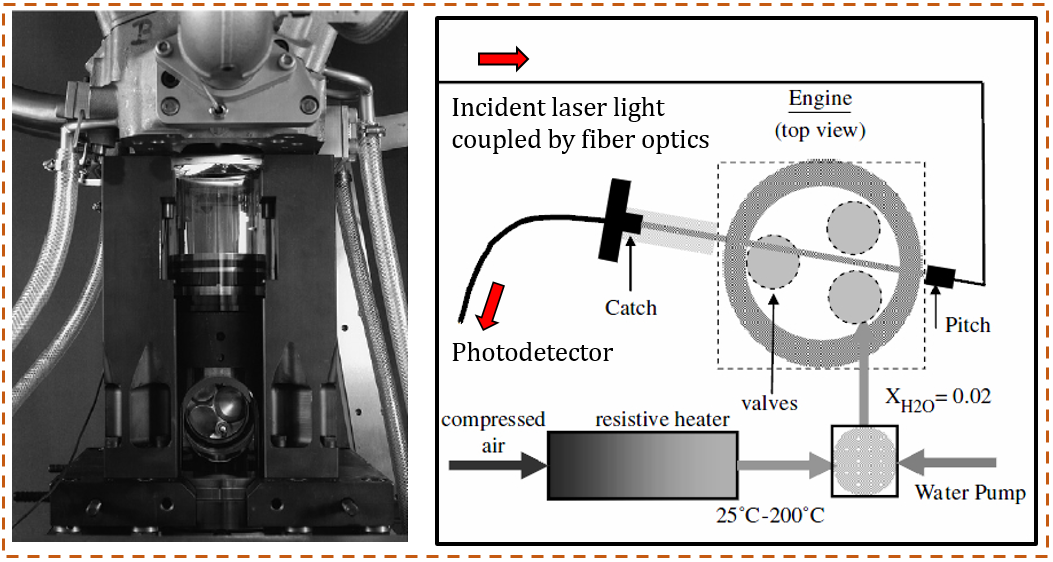
\includegraphics[width=0.75\textwidth]{fig/ch1_fig5.png}
        \caption{Left: an optical HCCI engine at Sandia National Laboratories; Right: a schematic of the fiber-optic-based LOS sensor for the temperature and $H_2O$ measurements in HCCI engine. Figure adapted from Mattison et al. \cite{Mattison2007}.}
    \label{fig:ch1_2}
\end{figure}

\begin{figure}[ht]
    \centering
        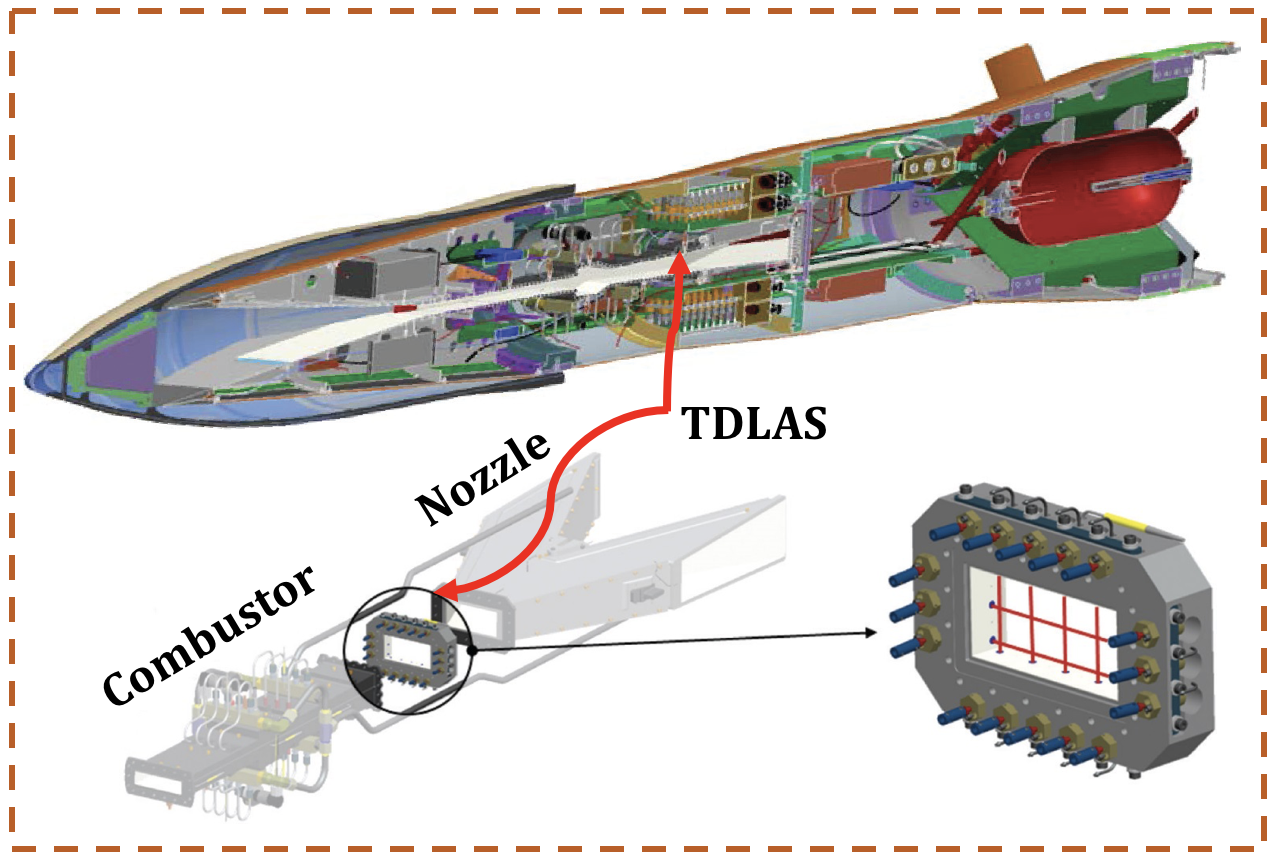
\includegraphics[width=0.6\textwidth]{fig/ch1_fig6_v2.png}
        \caption{Schematic of in-flight TDLAS sensor with 8 lines-of-sight in the HIFiRE 2 scramjet. Figure adapted from Jackson et al. \cite{Jackson2015}.}
    \label{fig:ch1_3}
\end{figure}


\subsection{Single-ended LAS probes}
Several researchers have developed single-ended probe-based LAS sensors to study combustion within internal combustion (IC) engines \cite{Melin2017, RIEKER20073041, Jeffries2010, Witzel2013, Bürkle2018}. Rieker et al. \cite{RIEKER20073041} acquired measurements of temperature and $H_2O$ concentration with a spark-plug-embedded probe in IC engines. Measurements were able to be made a temperatures from 500 to 1050 $K$ and pressures from 1 to 50 $atm$ with a bandwidth of 7.5 $kHz$. Rein et al. \cite{Rein:10} developed a Fourier Transform Spectroscopy (FTS) technique to get absorption spectra and measure temperature and water concentration using a optical spark plug probe (OSSP). Fig. 1.4 illustrates a schematic of a fiber-optic spark plug probe in detail. The incident laser beam passes through a sapphire window into the probe housing, which has channels to let combustion gases pass through. The laser light is transmitted through absorbing gases and reflected by a gold mirror on the probe. The transmitted beam is then collected by a mutlimode fiber which directs the light to a photodetector. This probe penetrates 5.3 $mm$ into the cylinder and provides an optical path length 10.6 $mm$ due to the double pass. Spark plugs with a single-ended probe-based sensor can be customized with the same specifications as industrial-type spark plugs and applied in production engines \cite{Jeffries2010}. Single-ended probe-based sensors enable measurements of gas properties to be acquired in environments with extremely limited optical access. However, the probe surface is known to perturb the local temperature and velocity field due to heat transfer losses and mechanical obstacles. As a result, this approach is somewhat invasive.

\vspace{30mm}

\begin{figure}[ht]
    \centering
        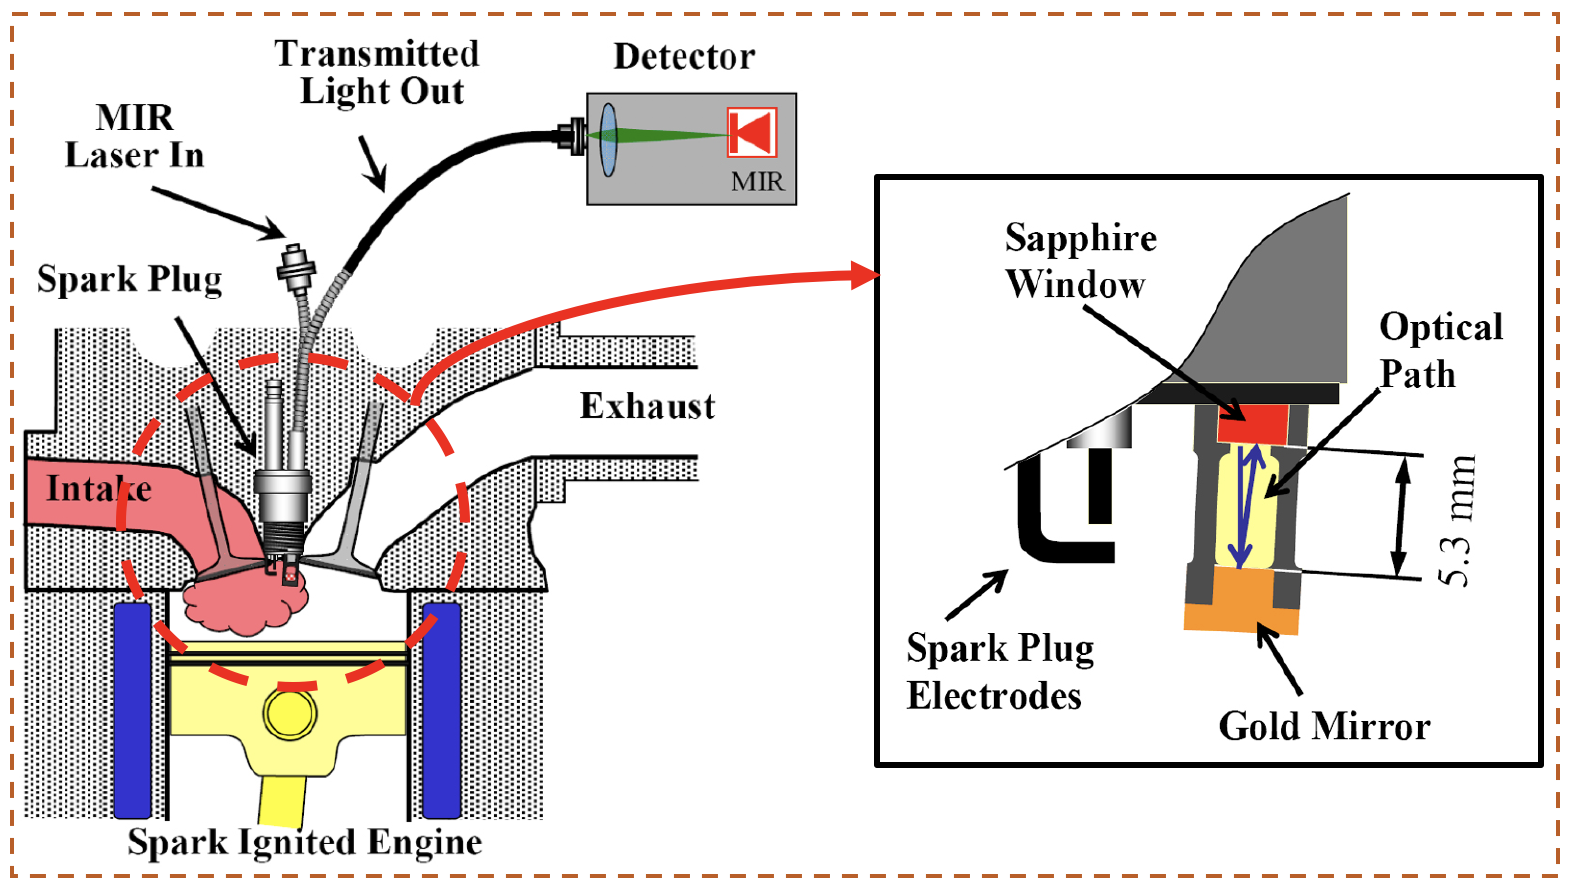
\includegraphics[width=0.7\textwidth]{fig/ch1_fig3.png}
        \caption{Left: A spark-plug optical probe used to provide mid-infrared absorption measurements of temperature and $H_2O$ in cylinder; Right: detailed schematic of the fiber-optic probe. Figure adapted from Jeffries et al. \cite{Jeffries2010}.}
    \label{fig:ch1_4}
\end{figure}

\subsection{Single-ended, backscattering-based LAS sensors}
Development of single-ended backscattering-based sensors have been a popular area of ongoing research due to their non-intrusive nature and applicability to environments with extremely limited optical access. This type of sensor is capable of standoff or remote measurements by collecting laser light that is backscattered off native surfaces. Recently, Goldenstein et al. \cite{Goldenstein:16} developed a single-ended near-IR TDL sensor for stand-off measurements of gas properties using WMS techniques. In this sensor, a lens and fiber bundle were packed in a lens tube with 25.4 $mm$ diameter. This sensor achieved collection efficiencies from 1 to $10^4$ parts-per-million (ppm) at a stand-off distance between 10 $m$ to 10 $cm$. Melin et al. \cite{Melin2017} made use of a backscattering-based single-ended LAS sensor to acquire water vapor measurements at 10 $kHz$ in a HCCI engine. Most recently, Peng et al.  \cite{Peng:16} demonstrated the first single-ended LAS sensor employing mid-IR wavelengths to provide measurements of $H_2O$, $CO$ and $CO_2$ simultaneously (see Fig. 1.5). Later this sensor was used to characterize a rotating detonation engine \cite{Peng2018}.


\begin{figure}[ht]
    \centering
        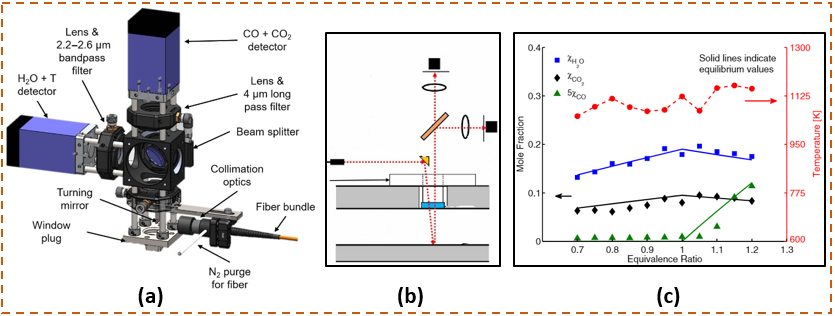
\includegraphics[width=1\textwidth]{fig/ch1_fig4.png}
        \caption{(a) CAD rendering of the single-ended sensor optical architecture; (b) a schematic of the optical path in the single-ended sensor architecture; (c) average temperature and $H_2O$, $CO$ and $CO_2$ mole fractions as a function of equivalence ratio. Figures adapted from Peng et al. \cite{Peng:16}.}
    \label{fig:ch1_5}
\end{figure}

\section{TDLAS of $H_2O$ Transitions in the Near-IR}
The use of LAS sensors relies on spectroscopic knowledge of the selected transitions of the target species. In practical applications, the detection limit of an absorption sensor depends on the transition strength or linestrength of the targeted transitions as this is the primary property that governs the amount of light absorbed by the target species. Water has relatively strong transitions in the near-IR since its vibrations are highly anharmonic which makes it well suited for detection via near-IR TDLs. $H_2O$ is also an attractive combustion species to study since it is one primary reaction product and an indicator of combustion efficiency (especially for $H_2$-fueled engines). Therefore, $H_2O$ has become one of the most widely used target species in LAS sensors. Fig. 1.7 illustrates the absorption spectrum of $H_2O$ in the near-IR and mid-IR. Experiments presented in this thesis (Chapter 4) focuses on demonstrations of LAS sensors operated in the near-IR (near 1400 $nm$). This enabled use of robust telecommunication grade tunable diode lasers and fiber optics which facilitated the design and fabrication of a new SE-LAS sensor. Further, the wavelength of these TDLs can be tuned by varying the laser current which facilitates the use of scanned-wavelength direct-absorption techniques and wavelength-modulation spectroscopy techniques. 

%As a near-IR hardware, distributed-feedback (DFB) lasers are one of the most applied lasers for LAS sensors. The laser can be tuned by a injection current over some wavelength ranges, which plays an important role in LAS techniques (Chapter 2 and 3). DFB tunable diode lasers (TDL) are capable of their ease if operations, low cost, wavelength stability, and customized tunability over a wide range of wavelengths (760 nm to 3$\mu m$) \cite{Goldenstein2017}.
\vspace{5mm}

\begin{figure}[ht]
    \centering
        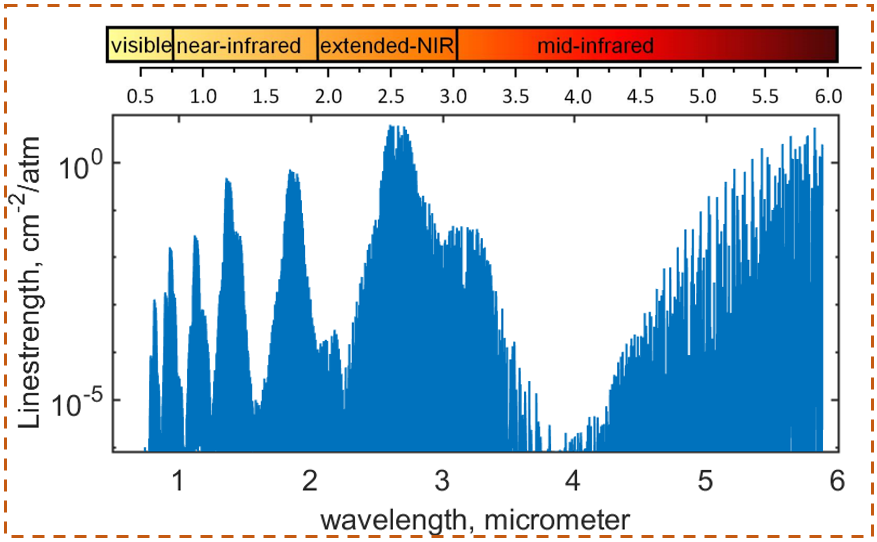
\includegraphics[width=0.7\textwidth]{fig/ch1_fig7.png}
        \caption{Strength of $H_2O$ absorption transitions in the NIR and mid-IR regions. Calculations were performed using the HITRAN 2012 database \cite{2013JQSRT.130....4R}.}
    \label{fig:ch1_7}
\end{figure}

%Applications of three types of LAS sensors: (a) line-of-sight sensor in engine measurements from []; (b) spark-plug-mounted probes from []; (c) mide-IR single-ended backscatter sensor from native surfaces in a combustor from []

\section{Outline of Thesis}
This dissertation is arranged to describe: 1) the fundamentals of absorption spectroscopy and WMS techniques and 2) the design and validation of a novel SE-LAS sensor architecture capable of providing measurements of temperature and $H_2O$ in combustors.

\begin{itemize}
\item \textbf{Chapter 2} presents the fundamental theory of laser-absorption spectroscopy and related techniques including direct absorption and WMS. 
\end{itemize}

\begin{itemize}
\item \textbf{Chapter 3} describes the operating principles of the wavelength-modulation spectroscopy techniques used in the SE-LAS sensor.
\end{itemize}

\begin{itemize}
\item \textbf{Chapter 4} describes the design and application of a SE-LAS sensor for temperature and $H_2O$ measurements. Two experiments were conducted to demonstrate the SE-LAS sensor: (1) fixed-WMS measurements during a transient ignition blast, and (2) scanned-WMS measurements over 30-minute period with the burner operating at quasi-steady-state. Results are compared with those from a line-of-sight sensor to validate the accuracy of the SE-LAS sensor.
\end{itemize}

%\begin{itemize}
%\item \textbf{Chapter 5} demonstrates singled-ended $H_2O$ sensing for temperature and water concentration in the after-treatment of a Cummins exhaust system located in Herrick Laboratories. A scan-WMS measurement is performed between downstream of diesel particulate filter (DPF) and inlet of selective catalytic reduction (SCR). Results are compared with those from a thermocouple and simulation software. Measurements are taken in the condition with and without urea injection respectively.
%\end{itemize}

\begin{itemize}
\item \textbf{Chapter 5} discusses the conclusions resulting from this work and some potential future potential research for SE-LAS sensing.
\end{itemize}
